%!TEX encoding=UTF-8 Unicode
\chapter{Collecting fine grain memory traces}
\label{chap:moca}

\gls{Tabarnac} manages to keep it's overhead reasonable by two means.
First it sees the memory at the granularity of the page, loosing any information about the internal use of a page.
While this is enough to debug issues specific to \gls{NUMA}, it is not \emph{detailed} enough to build a map of the memory accesses.
Second, it does not collect any temporal information, reducing the size of its trace and avoiding to maintain temporal order.
An instrumentation similar to \gls{Tabarnac} but with temporal information with a finer grain than the page would have a considerable overhead.
Therefore it is required to find a lighter mean to collect memory traces.
This chapter presents \gls{Moca}, a memory trace collection system that  relies on an \gls{OS} level mechanism called page fault interception and injection.
\gls{Moca} addresses the challenge of collecting \emph{detailed}, \emph{precise} and \emph{complete} traces, that is with temporal information.

This work is the subject of two Inria research reports~\cite{Beniamine15Memory,Beniamine16Moca} and has been submitted at \gls{CCGRID} 2017.
\gls{Moca} is distributed under the \gls{GPL} license: \url{https://github.com/dbeniamine/Moca}.

This chapter presents first the main components of \gls{Moca} in \sect{moca-components}.
Then we present some background knowledge required to understand \gls{Moca} design in \sect{moca-bg}.
After that we discuss the implementation details of \gls{Moca} \gls{Linux} kernel module in \sect{moca-design}.
Then we present an experimental validation including an extensive comparison with existing memory trace collection tools in \sect{moca-expe}.
Finally we provide our conclusions about memory traces collection in \sect{moca-cncl}.

\section{Moca components}
\label{sec:moca-components}

\gls{Moca} consist of a Linux kernel module that can be loaded at runtime,  a script in charge of both loading this module with the proper parameters and launching the monitored application on the user behalf and an optional context library able retrieve data structures information.
It neither relies on architecture specific technologies such as \gls{AMD} \gls{IBS} or \gls{Intel} \gls{PEBS}, nor on architecture dependent kernel code, kernel patch or kernel modifications.
Therefore it is portable and can be run on any Linux kernel from the $3.0$.

When the user wishes to retrieve data structure informations, \gls{Moca} runs the application twice with virtual address space randomization disabled.
The first time, the application is run with the context library preloaded but without the \gls{Linux} kernel module.
At the opposite, during the second run, only the \gls{Linux} kernel module is loaded.
This library is a port of the one used by \gls{Tabarnac} without the dependencies to \gls{Pin}.
It reads static data structures information in each executed binary file and stores data about structures larger than one page.
It also intercepts all calls to \texttt{malloc} family functions and names these calls according to their stack trace and retrieve stacks from the file \texttt{/proc/<pid>/maps}.
Naming the data structures by call stack instead of by looking at the source code is an improvement, as some code uses temporary pointers for allocations.
\gls{Moca} and the library are run separately as it would be costly for \gls{Moca} to check if each intercepted access has been triggered inside the context library.
Our context library is lightweight, the added cost is the cost of a regular execution added to a small constant overhead for each binary opened and each allocation performed.
Thus the overhead of using \gls{Moca} and the library is basically \gls{Moca} overhead plus one time the normal execution time.

\section{Background knowledge}
\label{sec:moca-bg}

As explained in \chap{mem}, in recent Linux kernel, physical memory pages are lazily allocated to page frames during the execution.
The first access to a page in the virtual address space triggers a page fault.
To handle this page fault, Linux allocates a physical page to the requested page frame.
Such a page fault can also be triggered when a thread access a shared page modified by another thread.
\gls{Linux} provides the possibility to intercept these page faults.
Page faults interception is an efficient mean to collect information about memory usage at the run time.
Such a mechanism has been used in several existing works : in parallel garbage collectors~\cite{Boehm91Mostly}, in memory checkpointing~\cite{Heo05Spaceefficient} or in the domain of virtualization to provide the hypervisor with information about the memory usage of the guest \gls{OS}~\cite{Jones06Geiger}.
However, page faults only occur when caused by predetermined events in the system (copy-on-write, paging, ...).
Thus, intercepting existing page faults at a relatively low frequency do not provide the precision required for a thorough analysis.
To improve this method, it is also possible to fake invalid pages at regular intervals in order to generate false page faults~\cite{Bae12Dynamic,Diener13CommunicationBased} at a higher frequency than regular ones.
These false page faults are just triggered during regular memory accesses, that would not have caused a page fault if the page were not faked as invalid.
The advantage is that they create additional events for the monitoring tool to collect, thus more \emph{precision}, but the tool must be able to identify faked invalid pages.
Fake page faults can be identified either by setting some bits of the \gls{PTE} that are not used by the \gls{OS}, yet this kind of hack is not portable and might interfere with runtimes or by maintaining the set of faked invalid pages in the monitoring tool.

Existing memory profiling tools do not use false page faults injection and only need to store the location of memory pages and the threads that access them.
As a consequence, they require a relatively small data structure in memory for their own usage.
\gls{Moca} is a new \emph{complete} memory trace collection system, based on page fault interception and false page faults injection, able to capture \emph{precisely} the temporal evolution of memory accesses performed by a multithreaded application.
To reach a satisfying \emph{precision}, \gls{Moca} has to maintain in memory both the trace data and the set of faked invalid pages.
Overall, storing and exploiting efficiently these data within the kernel space and outputting them in real time to the user space is a challenge and is the main contribution of our work.

\section{Design}
\label{sec:moca-design}

Two tasks are addressed by the kernel module included in \gls{Moca}.
The first one is to keep track of the set of pages accessed by the application during an elementary monitoring interval.
The second one is to manage the huge quantity of data produced by the trace collection within the kernel space in-between regular flushes toward the user space.
Of course, these two tasks should be as slightly intrusive as possible.

The remaining of this section discusses the design of \gls{Moca} \gls{Linux} kernel module as it is both the most important and the most complex part of \gls{Moca}.

\subsection{Page faults interception and injection}

\gls{Moca} collects \emph{complete} traces in the sense that the exact set of pages accessed by the application is deduced from the collected events at all times during the execution.
Thus, it is \emph{complete} at the page granularity.
Other information such as exact addresses and access times are a sample of the set of all the accesses.

\gls{Moca} is built upon the possibility to register an additional callback on Linux page faults.
Nevertheless, a page fault does not occur at each memory access.
To monitor memory accesses during the course of the execution, we need to reenable a page fault similar to the first access, but performed on a regular basis and on behalf of \gls{Moca}.
In other words, we need to inject false page fault by periodically marking as \emph{not present} the pages accessed by the application.
In Linux terminology, marking means that the next access to the page will trigger a page fault which will have to be handled, in this case, by a handler contained in \gls{Moca}.

This method has several advantages over hardware sampling or instrumentation.
First, it provides a superset of all the memory accesses, because it guarantees that each page accessed by the monitored application will fault once and will be traced.
Second, at the end of each monitoring interval, we know the exact set of accessed pages from which we deduce a superset of actual memory accesses.
This comes in addition to the fact that each false page fault generated provides \gls{Moca} with exact information about one memory access.
This means that \gls{Moca} also performs a sampling of all the memory accesses at the granularity of the Byte.
Because it is designed to manage large chunks of trace data within the kernel space, it also stores all the details about these samples in the collected trace.

\gls{Moca} differs from instruction sampling because it is not necessary to increase the monitoring frequency of \gls{Moca} to collect a \emph{complete} trace.
On the contrary, when using instruction sampling, if the pages of the application are accessed in an unbalanced manner, it is necessary to increase the sampling frequency to get a precise picture of the memory working set of the application.
Nevertheless, there can be no guarantee that a chosen sampling frequency will result in a trace that contains all the pages on which the application works.

\gls{Moca} also differs from instrumentation based tools because, just as in the case of sampling, memory accesses that are not collected in the trace are not trapped at all by a false page fault.
Furthermore, the remaining memory accesses, which are collected, are trapped using a hardware mechanism and Linux kernel probes.
Both are lightweight mechanisms, which means that the overall instrumentation overhead of \gls{Moca} is likely to be low.
Indeed, instrumentation based methods often work at a high granularity, collecting few information, in order to keep their naturally high overhead in control.

\subsection{Internal design}

During the execution, our \gls{Linux} kernel module needs to store three kinds of information:

\begin{enumerate}
    \item The set of \emph{tasks} (Linux internal representation of threads and processes) which are
monitored.
    This is necessary because page faults will also be triggered by tasks which do not belong to the monitored application.
    \item The set of all page faults which have been injected by \gls{Moca}, required to distinguish false page faults from regular ones, because their handling differs.
        False page fault could also be identified by setting some bits of the \gls{PTE} that are not used by the \gls{OS}.
        While this solution avoid to maintain the set of false page fault, it is a hack not portable and could interfere with a runtime.
    \item The set of addresses recently accessed by each task, this set correspond to the actual memory trace.
        It is required to keep it in kernel space as we need to reinject these false page faults at the end of each monitoring interval.
        Afterwards, this set is transferred to the user space by a dedicated process and appended to the resulting trace.
\end{enumerate}

These sets of data are stored in hashmaps.
The \gls{Linux} kernel provides some helpers to manage such hashmaps, still these maps generate an allocation each time we add an element to it.
Therefore we implemented generic pre-allocated hashmaps in our kernel module.
As memory space is restricted in the kernel space, these hashmaps are not statically allocated, but they only call the \emph{kmalloc} function during their initialization.
Furthermore, they are initialized as soon as possible which means at the beginning of the execution for the two first sets, and each time a new thread is created for the third.
As \gls{Moca} does not have any a priori knowledge of the monitored application, it allocates huge hashmaps.
If the monitored application has a considerable memory footprint they might be too small, in this case, \gls{Moca} will drop a part of the trace and notify the user that it is incomplete.
The user can then either monitor its application on a smaller input or  use \gls{Moca} parameters to change the size of these hashmaps.

The two first sets of data are read at each page fault but rarely written, only when a new task of the monitored application triggers its first page fault or when \gls{Moca} generate new false page faults.
We can protect them with Linux kernel built-in \emph{rwlocks}.
The third type of information is the actual trace, divided, for each task, in a private set of \emph{chunks}.
A chunk is the set of accesses that have been collected during the monitoring time interval and is implemented as a hashmap.
Chunks provide a discretization of time, each chunk embed two timestamp to mark its temporal bounds.
To reduce the volume of information stored, the accesses are not timestamped.
However, the arrival order in the chunk is preserved in the final trace file.

\begin{figure}[htb]
    \centering
    \pgfdeclarelayer{background}
\pgfdeclarelayer{bg1}
\pgfdeclarelayer{foreground}
\pgfsetlayers{background,bg1,main,foreground}

\definecolor{logcolor}{HTML}{FDAE61}
\definecolor{moncolor}{HTML}{FF000A}
\definecolor{pfcolor} {HTML}{3B8ECC}
\definecolor{callcolor}{HTML}{FFFFBF}
\definecolor{dtcolorL}{HTML}{ABD9E9}
\colorlet{dtcolor}{dtcolorL!25}

\tikzstyle{handler} = [rectangle, draw, fill=callcolor,
text width=4em, text badly centered]
\tikzstyle{handlerI} = [diamond, text badly centered]
\tikzstyle{data} = [rectangle, draw, fill=dtcolor,
text width=4em, text centered, rounded corners]
\tikzstyle{Chunk} = [rectangle, draw,rounded corners]
\tikzstyle{dataL} = [rectangle, draw, fill=dtcolorL,
text width=4em, text centered, rounded corners]
\tikzstyle{entity} = [draw, ellipse, text centered,
text width=5em]
\tikzstyle{line} = [very thick,align=center]
\tikzstyle{pf} = [fill=pfcolor,solid]
\tikzstyle{log} = [fill=logcolor,dotted]
\tikzstyle{mon} = [fill=moncolor,dashed]
\tikzstyle{monA} = [-latex,line,dashed,moncolor]
\tikzstyle{pfA} =  [-latex,line,solid,pfcolor]
\tikzstyle{pfAI} =  [line,solid,pfcolor]
\tikzstyle{logA} = [-latex,dotted,line,logcolor]

\tikzset{
  basic box/.style = {
    shape = rectangle,
    draw,
    rounded corners},
  filled box/.style = {
    shape = rectangle,
    draw  = #1,
    fill  = #1,
    rounded corners},
  header node/.style = {
    %Minimum Width = header nodes,
    font          = \strut\large\ttfamily,
    text depth    = +0pt,
    fill          = #1,
    draw},
    header/.style n args={2}{%
    inner ysep = +1.5em,
    append after command = {
      \pgfextra{\let\TikZlastnode\tikzlastnode}
      node [header node=#2] (header-\TikZlastnode) at (\TikZlastnode.north) {#1}
      %node %[span = (\TikZlastnode)(header-\TikZlastnode)]
       % at (fit bounding box) (h-\TikZlastnode) {}
    }
  },
  footer node/.style = {
    %Minimum Width = header nodes,
    font          = \strut\large\ttfamily,
    text depth    = +0pt,
    fill          = #1,
    draw},
    footer/.style n args={2}{%
    inner ysep = +1.5em,
    append after command = {
      \pgfextra{\let\TikZlastnode\tikzlastnode}
      node [header node=#2] (header-\TikZlastnode) at (\TikZlastnode.south) {#1}
      %node %[span = (\TikZlastnode)(header-\TikZlastnode)]
       % at (fit bounding box) (h-\TikZlastnode) {}
    }
  },
  hv/.style = {to path = {-|(\tikztotarget)\tikztonodes}},
  vh/.style = {to path = {|-(\tikztotarget)\tikztonodes}},
  fat blue line/.style = {ultra thick, blue}
}



\begin{tikzpicture}[font=\small,scale=.73, each node/.style={minimum width=1em}]
    % Node placement
    \begin{pgfonlayer}{foreground}
        \node [Chunk] (ch3) at (0,0)        {Chunk3 empty};
        \node [Chunk] (ch2) at (0,-1)       {Chunk2 current};
        \node [Chunk] (ch1) at (0,-2)       {Chunk1 ending};
        \node [Chunk] (ch0) at (0,-3)       {Chunk0 completed};
        \node [Chunk] (cur) at (2.5,-1.5)   {current};

        \draw [line,->] (cur.north) |- (ch2.east);
    \end{pgfonlayer}

    \node [fit=(cur) (ch0) (ch1) (ch2) (ch3),filled box=dtcolor,
    header={Trace (1 Task)}{dtcolor!50}] (Tr) {};

    \node [data] (PfL) at (5,-1) {False Page fault map};
    \node [data] (TL)  at (8,-1) {Tasks map};


    \node[handler] (Flh) at (1,-5.5) {Read callback};
    \node[handler] (PfH) at (7.5,-4.5) {page fault handler};


    \node[entity,log] (F) at (0.9,-8) {Logging Process (userspace)};
    \node[entity,mon] (M) at (5.5,-8) {Monitor thread (kernel)};


    \begin{pgfonlayer}{background}
        \node[fit=(F) (M) (cur) (Flh) (PfH) (Tr) (PfL)(TL),header={Moca}{white},basic box] (Moca) {};
    \end{pgfonlayer}

    \node[entity,text width=5.5em,pf] (T) at (7,-12) {Tasks\\(user/kernel\\thread/process)};

    \node [dataL] (pgt)  at (5,-14.5)     {Page table (kernel)};
    \node [dataL] (proc) at (2,-14.5)     {/proc file (kernel)};
    \node [dataL] (file) at (-1,-14.5)     {File (userspace)};

    \begin{pgfonlayer}{background}
        \node[fit=(file) (proc) (pgt) (T),footer={Linux}{white} ,basic box=red,
        %below=1.5em of Moca
    ] (Linux) {};
    \end{pgfonlayer}

    % Edges

    %% Loging process
    \path[logA] (F.south) edge[in=140,out=270] node[right] {read} (proc.west);
    \path[logA] (proc.north) edge[in=-20,out=120]  node[pos=.2,right] {triggers} (Flh.east);
    \path[logA] (Flh.north) edge[out=90,in=270] node[pos=.2,left] {read write} (ch0.south);

    \path[logA] (Flh.west) edge[in=100,out=230] node[pos=.1,left] {write} (file.north);

    % Page faults
    \path[pfA] (T)   edge[out=70,in=-70] node[pos=.05,right] {triggers} ($(PfH.south)+(1,0)$);

    \coordinate (inv) at (5.25,0.5);
    \path[pfAI] (PfH.north) edge[out=135,in=0] (inv);
    \path[pfA]  (inv)     edge[out=180,in=20] node[pos=.1,above] {write} ($(ch2.east)+(0,0.2)$);

    \path[pfA] (PfH.north) edge node[right] {read \\ (write)} (TL.south);
    \path[pfA] (PfH.north) edge[out=160,in=310] node[pos=.8,right] {read} ($(PfL.south)+(0.2,0)$);

    \coordinate (inv2) at ($(M.south)-(0,0.5)$);
    \path[pfAI] ($(PfH.south)+(0.5,0)$) edge[out=-60,in=0] (inv2);
    \path[pfA] (inv2) edge[out=180,in=120] node[pos=.35,right] {read\\write} (pgt.north);

    %Monitor
    \path[monA] (M.north) edge[out=70,in=290] node[pos=.2,right] {write} (PfL.south);
    \path[monA] (M.north) edge[out=110,in=-30] node[pos=.6,left] {write} (cur.east);
    \path[monA] (M)  edge[out=-130,in=110] node[pos=.8,left] {write} ($(pgt.north)-(.6,0)$);

    \path[monA] (M.north) edge[out=170,in=-10] node[pos=.5,left] {read} (ch1.east);
\end{tikzpicture}


    \caption{Interactions betweens Moca and Linux.}
    \label{fig:moca}
\end{figure}

The discretization of time, materialized as a sequence of chunks, is useful as it let the different components of \gls{Moca} work concurrently on different chunks.
Indeed, the traced program always works on \emph{current} chunks, one for each core, while the logging daemon, which flushes the trace from memory to permanent storage works on \emph{completed} chunks.
A monitoring kernel thread, manages the progress of this logical time.
It periodically wakes up, marks the current chunks as \emph{ending} and invalidates all the pages they reference.
Once all pages of the \emph{ending} chunks have been invalidated, it marks these chunks as \emph{completed}.
Finally, the logging process flushes \emph{completed} chunks to the filesystem at a lower rate, in order to reduce the overhead of I/Os requests, and recycle them as empty places for upcoming chunks.
%\GH{Pourquoi à un rythme moins élevé ??? En théorie des files d'attentes ce genre de choses = débordement...}
%\DB{L'idée était de limiter la bande passante disque, et croiser les doigt pour que les files soient assez grosses \ldots Il faudrait essayer un logging interval très petit sur MG.}
%\GH{On peut aussi éventuellement rajouter les trois mots précédents, histoire de dire que le but est de factoriser les requêtes, pas de remplir la mémoire}
 \fig{moca} depicts the interaction between the different processes and threads of \gls{Moca}, its data structures and Linux.

Eventually, \gls{Moca} generates one csv file, each line of this file describe one access giving its physical and virtual address, the number of read and writes captured, a bitmask indicating on which CPU the access occurred, the start and end timestamp of its chunk and the internal identifier of the task which triggered it.
A set of access sharing the same timestamps and task identifier correspond to a chunk.
The order of accesses inside a chunk is preserved.

\begin{algorithm}[htb]
    \caption{Monitoring thread algorithm}
    \label{alg:monTh}
    \begin{algorithmic}[1]
        \While{\Callp{NotFinished}{}}
            \ForAll{t in \Callp{MonitoredTasks}{}}
                \State \Callp{EndCurrentChunk}{t}
                    \ForAll{Addr in \Callp{PreviousChunk}{t}}
                        \State \Callp{WriteLockPF}{}
                        \State \Callp{AddFalsePF}{Addr}
                        \State \Callp{WriteUnlockPF}{}
                    \EndFor
                \State \Callp{MarkPreviousChunkFinished}{t}
            \EndFor
            \State \Callp{sleep}{MonitorThreadWakeUpInterval}
        \EndWhile
    \end{algorithmic}
\end{algorithm}

The monitoring thread, which is a kernel thread, that uses the \alg{monTh}, is in charge of enabling false page faults destined for \gls{Moca}.
It performs its task by removing the \texttt{PRESENT} flags from the \gls{PTE} that corresponds to each recently accessed addresses.
Of course, the shorter is the period between two wakeups, the more precise the trace is.
This period is called \emph{monitor thread wakeup interval} (or \emph{monitoring interval}).
But invalidating all the recently accessed pages takes time as it requires to take a write lock on the page faults hashmap.
This write lock delays any pending false page fault in the monitored application.
Thus the wakeup frequency of the monitoring thread cannot be too high, otherwise its action becomes too intrusive.
The \texttt{MonitorThreadWakeUpInterval} \gls{Moca} parameter lets the user change the default setting that we have empirically chosen after a few experiments.

\begin{algorithm}[htb]
    \caption[Moca Logging daemon algorithm.]{Logging daemon algorithm.\\
        \footnotesize{Note that no locks are required to work on completed chunks.}}
    \label{alg:moca-log}
    \begin{algorithmic}[1]
        \While{\Callp{NotFinished}{}}
        \ForAll{t in \Callp{MonitoredTasks}{}}
                \ForAll{c in \Callp{FinishedChunks}{t}}
                \State \Callp{WriteTraceToDisk}{c}
                \State \Callp{ReinitChunk}{c}
                \EndFor
            \EndFor
            \State \Callp{sleep}{LoggingDaemonWakeupInterval}
        \EndWhile
    \end{algorithmic}
\end{algorithm}

The logging daemon, that uses \alg{moca-log}, is a userspace process which periodically reads \texttt{/proc} pseudo files used by \gls{Moca} kernel module to export its data to userspace.
Those reads trigger a callback method in our tool which flushes completed chunks from memory to disc.
As it works on completed chunks, it does not directly interfere with the normal application execution.
Especially, no lock is required to access to these completed chunks, and, as it mostly generates disc I/O, it does not compete much for CPU.
\gls{Moca} has just to wake him up sufficiently often so that the kernel module does not run out of free space to store upcoming chunks.

%\begin{algorithm}[htb]
%    \caption{Page fault handler}
%    \label{algo:PageFault}
%    \begin{algorithmic}[1]
%        \Function{HandleFault}{task t,void *addr, int type}
%            \If {\Callp{IsNotMonitoredTask}{t}}
%                \If {!\Callp{AddToMonitoredIfNeeded}{t}}
%                    \State \Return \Comment{Resume page fault}
%                \EndIf
%            \EndIf
%            \State \Callp{AddToChunk}{t,addr, type}
%            \Comment{Trace the access}
%            \State \Callp{ReadLockPF}{}
%            \State \Callp{TryFixFalsePageFault}{addr}
%            \State \Callp{ReadUnlockPF}{}
%            \State \Callp{UpdateClock}{}
%            \State \Comment{Resume page fault. If a fix occurred, Linux will
%                silently abort the page fault}
%        \EndFunction
%    \end{algorithmic}
%\end{algorithm}

\begin{figure}[htb]
    \centering
    %!TEX encoding=UTF-8 Unicode

\tikzstyle{decision} = [rectangle, draw, fill=orange!30,text centered,
text width=6.5em]
\tikzstyle{mblock} = [rectangle, draw, fill=blue!25,text centered, rounded corners, node distance=3cm, minimum height=3em]
\tikzstyle{lblock} = [rectangle, draw, fill=blue!10, text centered, rounded corners, node distance=3cm, minimum height=3em]
\tikzstyle{line} = [draw, -latex,thick]

\tikzset{
  basic box/.style = {
    shape = rectangle,
    draw,
    rounded corners},
  header node/.style = {
    %Minimum Width = header nodes,
    font          = \strut\large\ttfamily,
    text depth    = +0pt,
    fill          = #1,
    draw},
    header/.style n args={2}{%
    inner ysep = +2em,
    append after command = {
      \pgfextra{\let\TikZlastnode\tikzlastnode}
      node [header node=#2] (header-\TikZlastnode) at (\TikZlastnode.north) {#1}
      %node %[span = (\TikZlastnode)(header-\TikZlastnode)]
       % at (fit bounding box) (h-\TikZlastnode) {}
    }
  },
}

\newcommand*{\StrikeThruDistance}{0.15cm}%
%\newcommand*{\StrikeThru}{\StrikeThruDistance,\StrikeThruDistance}%
\tikzset{strike thru arrow/.style={
        decoration={markings, mark=at position 0.5 with {
            \draw [black, very thick,solid,-]
                    ++ (-\StrikeThruDistance,-\StrikeThruDistance)
                    -- ( \StrikeThruDistance, \StrikeThruDistance);
            \draw [black, very thick,solid,-]
                    ++ ( \StrikeThruDistance,-\StrikeThruDistance)
                    -- ( -\StrikeThruDistance, \StrikeThruDistance);
                } },
                    postaction={decorate},
                                    }
        }

    \begin{tikzpicture}[scale=0.8]

        \node [lblock]   (pf)  at (0,0) {PageFault(task, @)};

        \node [lblock]   (hpf)  at (0,-5) {HandleFault(task,@)};

        \node [lblock]   (resume)   at (0,-9){Resume execution};

        \uncover<2->{
            \node [mblock]   (pfi) at (10,0) {InterceptPageFault(task,@)};

            \node [decision] (mon) at (10,-2) {Is task monitored ?};

        }
        \uncover<3->{
            \node [decision] (shou) at (5,-3) {Should we monitor it ?};
            \node [mblock] (Add)  at (10,-5) {AddToChunk(task,@)};
        }

        \uncover<4->{
            \node [mblock] (Add1) at (5,-5) {Monitor(task)};
        }

        \uncover<5->{
            \node [decision] (sfix)     at (10,-7) {Is it a false page fault ?};
        }

        \uncover<6->{
            \node [mblock]   (fix)      at (10,-9) {FixFalsePageFault(task,@)};

        }
        \node[fit=(pfi) (shou) (fix),header={Moca}{white},basic box] (Moca) {};
        \node[fit=(pf) (hpf) (resume),header={Linux}{white},basic box] (OS) {};

        \only<1>{
            \draw [line] (pf) -- (hpf);
        }
        \path [line] (hpf) -- (resume);

        \only<2->{
            \path [line] (pf.south) -- ($(pf.south)+(0,-.4)$) --
            ($(pf.south)+(5,-.4)$)  -- ($(pfi.north)+(-5,.4)$) --
            ($(pfi.north)+(0,.4)$) -- (pfi.north);

            \draw [-latex, strike thru arrow,dashed] (pf) -- (hpf);

            \path [line] (pfi.south) -- (mon.north);
        }


        \only<3->{

            \path [line] (mon.west) -- node [pos=.2,above] {No} ($(mon)+(-5,0)$)
            -- (shou.north);
            \path [line] (mon.south) -- node [pos=.2,right] {Yes} (Add.north);
        }
        \only<4->{

            \path [line] (shou.west)  -- node [pos=.9,above] {No} ($(shou)+(-2.25,0)$)
            -- ($(shou)+(-2.25,-.5)$) -- ($(hpf)+(0,1.5)$) -- (hpf.north);

            \path [line] (shou.south) -- node [right] {Yes} (Add1.north);

            \path [line] (Add1.south) -- ($(Add1.south)+(0,-.5)$)
            -- ($(Add1.south)+(2,-.5)$) -- ($(Add.north)+(-3,1)$)
            -- ($(Add.north)+(0,1)$) -- (Add.north);

        }
        \only<5->{
            \path [line] (Add.south) -- (sfix);

        }\only<6->{
            \path [line] (sfix.west) -- node [pos=.1,above] {No}
            ($(sfix)+(-7.25,0)$) -- ($(sfix)+(-7.25,3.5)$)
            -- ($(hpf)+(0,1.5)$) -- (hpf.north);

            \path [line] (sfix.south) -- node [right] {Yes} (fix.north);
        }
        \only<7->{
            \path [line] (fix.south) -- ($(fix.south)+(0,-.5)$)
            -- ($(fix.south)+(-7.25,-.5)$) -- ($(fix)+(-7.25,1.5)$)
            -- ($(resume)+(0,1.5)$) --(resume.north);
        }

    \end{tikzpicture}


% vim: et si sta lbr  sw=4 ts=4 spelllang=en_us


    \caption{Flow chart of Moca's page faults}
    \label{fig:fpf-flow}
\end{figure}

Each time a page fault occurs, it is trapped by the handler registered by \gls{Moca}.
As depicted by \fig{fpf-flow}, it first finds out if the task (thread or process) involved by the page fault is monitored or not.
If not, it has to check if the task is a child of a monitored task and, in this case, it starts monitoring it.
The check be done with a simple read lock on the hashmap containing the monitored tasks, the write lock is only taken if the task must be added.
This last case occurs only at the first page fault from a new monitored process or thread which is quite rare and usually occurs only at initialization time.
For instance, in the benchmarks used for the evaluation it happens $8$ times out of $5\times10^6$ accesses.
At the end of this phase, if the task is still not monitored, we let Linux handle the page fault as usual.

When a monitored task triggers a page fault, the access is first added to its current chunk.
For each access, \gls{Moca} stores the exact address, its type (read or write) and the CPU on which the fault occurred.
Then, it checks if the page fault has been injected by \gls{Moca} or if this is a legitimate page fault.
To do so, it needs to take a read lock on the false page fault hashmap.
In the first case, \gls{Moca} \emph{fixes} it by setting the \texttt{PRESENT} flag on the \gls{PTE}.
The hashmap entry indicating that the fault was injected by \gls{Moca} should then be removed, but this would required a write lock, so we only mark the hashmap entry as \texttt{BAD}.
\gls{PTE} are stored in \gls{PMD} themselves stored in \gls{PGD}, to write a flag on a \gls{PTE} it is required to take a lock at the \gls{PMD} level.
Thus, if two threads faults at the same page in parallel, they will be serialized at this step and only one of the thread will change this flag.
Therefore, it is safe to mark the page entry as \texttt{BAD} without holding the write lock.
When the monitoring thread, which already holds a write lock on this hashmap, injects false page faults it might run out of space.
In this case, it walks the hashmap freeing all \texttt{BAD} entries it enconters.
This lazy removal reduce the overhead of \gls{Moca} three different ways.
First, it avoid serializing page faults.
Then, it avoid removing entries when there are still enough room, which is highly probable as we allocate huge hashmaps independently from the memory footprint of the monitored application.
Finally, it enables recycling entries for page that are often accessed, speeding up the monitoring thread.

If a fix occurred in the \gls{Moca} handler, Linux silently aborts the page fault when it resumes its execution.
In the other case, it executes a normal page fault handling.
Each page fault increases an atomic clock that is used to timestamp the beginning and end of the chunks.
A race might occur if the monitoring thread enables a false page fault between the end of our handler and the end of Linux page fault handler.
To avoid that, \gls{Moca} stores for each CPU the last address that faulted, and does not clear it right away but at the end of the next chunk.

%All default values for the parameters that can influence either the accuracy of the trace or the
%overhead of the tool (such as the number and size of chunks, wakeup intervals
%for the monitoring thread and the logging process \ldots) can be overridden by the
%user. Nevertheless, reasonable defaults have been defined from the experimental study
%detailed in section~\ref{sec:expe-param}.

\section{Experimental validation}
\label{sec:moca-expe}

In this section, we compare \gls{Moca} and \gls{Tabarnac} to other existing memory analysis tools.
In a first time, we present their main differences in terms of portability and capabilities.
Then, we present two sequences of quantitative experiments, one that outlines the importance of the default parameters chosen for \gls{Moca} and the other that compares the precision and performance of all the tools.

\subsection{Methodology}

Our main experiments were run on  machines from \gls{Grid5000} \texttt{Edel}
cluster (Intel machines).
As some state of the art tools can only run on \gls{AMD} machines, we also ran
    some of the experiments on
    \texttt{StRemi} machine from \gls{Grid5000} grenoble.
    These machines hardware and software specifications%
    \footnote{\gls{Grid5000} provides an online hardware description:\\
       \url{https://www.grid5000.fr/mediawiki/index.php/Grenoble:Hardware\#Edel}
       \\\url{https://www.grid5000.fr/mediawiki/index.php/Reims:Hardware\#Stremi}}
    are summarized in \tbl{hw-moca}.

\begin{table}[htb]
    \centering
    \begin{tabular}{lllllllllll}
        \toprule
        & \multicolumn{5}{c}{\textbf{Hardware totals}}\\
        \cmidrule(lr){2-6}
        & Nodes & Threads & Vendor & Model & Memory \\
        \cmidrule(lr){2-6}
        \texttt{Edel}    & $2$ & $8$  & Intel & Xeon E5520      & \SI{24}{Gib} \\
        \texttt{StRemi} & $2$ & $24$ & AMD   & Opteron 6164 HE & \SI{48}{Gib} \\
        \midrule
        & \multicolumn{5}{c}{\textbf{Hardware per node}}\\
        \cmidrule(lr){2-6}
        & Cores & Threads & Frequency & L3 Cache & Memory \\
        \cmidrule(lr){2-6}
        \texttt{Edel}   & $4$  & $4$   & \SI{2.27}{Ghz}& \SI{8}{Mib}  & \SI{12}{Gib} \\
        \texttt{StRemi} & $12$ & $12$  & \SI{1.70}{Ghz}& \SI{12}{Mib} & \SI{24}{Gib}\\
        \midrule
        & \multicolumn{5}{c}{\textbf{Software}}\\
        \cmidrule(lr){2-6}
        & \multicolumn{2}{c}{Distribution} & Kernel &
            \multicolumn{2}{c}{Bios configurations} \\
        \cmidrule(lr){2-6}
        \texttt{Turing}   & \multicolumn{2}{c}{Debian Jessie} & Linux 3.16.0-4 &
            \multicolumn{2}{c}{No hyper threading} \\
        \texttt{Idfreeze} & \multicolumn{2}{c}{Debian Jessie} & Linux 3.16.0-4 &
            \multicolumn{2}{c}{No hyper threading}\\
        \bottomrule
    \end{tabular}
    \caption{Hardware and software configuration of the evaluation systems for Moca.}
    \label{tab:hw-moca}
\end{table}

\begin{table}[htb]
    \centering
    \begin{tabular}{lcccc}
        \toprule
         & \textbf{Moca} & \textbf{Tabarnac} & \textbf{Mitos} & \textbf{MemProf} \\
            \midrule
            \textbf{Design} & & & &\\
            \midrule
            Mechanisms   & Page faults  & Inst* & PEBS + Inst* & IBS \\
            Architecture & \textbf{Any} & Intel (AMD) & Intel & AMD   \\
            \midrule
            \textbf{Completeness} & & & &\\
            \midrule
            Trace Granularity & \textbf{Address} & Page          & \textbf{Address} & \textbf{Address} \\
            Superset          & \textbf{Page} & \textbf{Page} & None             & None             \\
            \midrule
            \textbf{Detail} & & & &\\
            \midrule
            Temporal data & \textbf{Yes} & No          & \textbf{Yes} & \textbf{Yes} \\
            CPU location  & \textbf{Yes} & No          & \textbf{Yes} & \textbf{Yes} \\
            Nature        & \textbf{Yes} &\textbf{Yes} & Yes**         & Yes**       \\
        \bottomrule
    \end{tabular}
    \caption[Comparison of different memory traces tools.]
    {Comparison of different memory traces tools.\\
        \footnotesize{
            *Inst: Instrumentation.\\
            **Type (Read/Write) must be deduced from the instruction name.
        }
    }
    \label{tab:tools-comp}
\end{table}


%For each experiment, we deployed the same \emph{Debian} \emph{Jessie} environment running a \texttt{Linux 3.16.0-4} on a machine with hyper threading disabled.
We disabled address space randomization to make the comparison between different traces more practical.
As our two evaluation machines do not have the same hardware, we limited the number of threads used by \gls{OpenMP} to $8$, that is the largest number of hardware threads available on both machines.

We evaluate \gls{Moca} and \gls{Tabarnac} by comparing them to the following state of the art tools. The first one,
\gls{Mitos}, is the tracing tool from \gls{MemAxes}~\cite{Gimenez14Dissecting} and relies on \gls{Intel} \gls{PEBS} technology.
The second one, \gls{MemProf}~\cite{Lachaize12MemProf}, is designed to analyze \gls{NUMA} performance issues and relies on \gls{AMD} \gls{IBS}.
The main differences between these memory profiling tools are summarized in \tbl{tools-comp}.

\begin{table}[htb]
    \centering
    \begin{tabular}{lrll}
        \toprule
        \textbf{Name} & \textbf{Footprint*} & \textbf{Description} & \textbf{Group} \\
        \midrule
        \IS & \SI{132}{Mib} & Integer Sort  &
        \multirow{4}{*}{Memory Intensive}\\
        \CG & \si{125}{Mib} & Conjugate Gradient & \\
        \MG & \si{508}{Mib}& Multi-grid & \\
        \FT & \si{398}{Mib}& Discrete 3D FFT & \\
        \midrule
        \UA & \si{112}{Mib}& Unstructured Adaptive mesh &
        \multirow{2}{*}{Unstructured} \\
        \DC & $1.46$Gib & Data Cube & \\
        \midrule
        \BT & \si{120}{Mib}& Block Tri-diagonal solver &
        \multirow{3}{*}{Pseudo Applications} \\
        \SP & \si{122}{Mib}& Scalar Penta-diagonal solver & \\
        \LU & \si{118}{Mib}& Lower-Upper Gauss-Seidel solver & \\
        \midrule
        \EP & \si{78}{Mib}& Embarrassingly parallel & CPU bound\\
        \bottomrule
    \end{tabular}
    \caption[Description of the \acrlong{NPB}.]{Description of the \acrfull{NPB}.\\
    \footnotesize{*Footprints: maximum memory used, measured with Valgrind tool: Massif}.}
    \label{tab:NPB}
\end{table}

In the following sections, all the tools are evaluated on each of the 10 \gls{NPB}~\cite{Jin99NPBOpenMP}, which are presented in \tbl{NPB}, according to the information available on the NASA website\footnote{
    \url{http://www.nas.nasa.gov/publications/npb.html}}.
In this table, we included the footprint of each benchmark, that is the maximum memory used, as reported by Valgrind's tool Massif.

In each experiment, \gls{Moca} and \gls{Tabarnac} were run with their default parameters,
except for the experiment about the influence of \gls{Moca} parameters.
For \gls{Moca}, their default values are: a wakeup interval of \SI{0.5}{s} for the logging process and \SI{50}{ms} for the monitoring thread.
Each point in each plot is the average of at least $30$ executions.
Along with each point, the error bars represent the standard error.

As explained in \chap{perf}, we distribute\footnote{
    See our experiment repository:
    \url{https://github.com/dbeniamine/Moca_expe}
} all the files needed to reproduce our experiments at three different levels:
The first level contains the filtered results (csv files) from the experiments along with the \texttt{R-markdown} scripts that generated the plots presented in this article, making possible the reproduction of our statistic analysis.
The second consists of the full raw traces generated by our experiments along with the scripts used to extract the filtered traces (csv files from the previous level) and the scripts used at the previous level to perform the analysis.
Finally, at the most comprehensive level, we provide a git repository that includes our deployment environment, dependencies to all the tools and files required and instructions that explain how to reproduce the experiment with or without access to \gls{Grid5000}.


\subsection{Moca validation}
\label{sec:expe-param}

Before comparing \gls{Moca} to existing tools, we need to evaluate the impact of the wakeup intervals (logging daemon and monitoring thread) on the trace \emph{precision} and on the overhead.
To do so, we ran the \IS benchmark instrumented by \gls{Moca} with a wakeup interval ranging from \SI{0.1}{s} to  \SI{0.9}{s} for the logging daemon and from \SI{20}{ms} to \SI{100}{ms} for the monitoring thread.
We decided to evaluate monitoring thread wakeup interval close to the \gls{Linux} scheduler interval \SI{50}{ms} as these events seems related to us.
Concerning the logging interval we need it to be longer than the previous one to limit the impact of \glspl{I/O}.
For each run, we measure \IS execution time and the number of accesses captured.
We have chosen \IS for this evaluation as it is one of the memory intensive out of the \gls{NPB} and quick experiments with other ones confirmed these results.
This experiment was run on a machine from the \texttt{Edel} cluster.

\begin{figure}[htb]
    \centering
    \begin{subfigure}{.73\linewidth}
        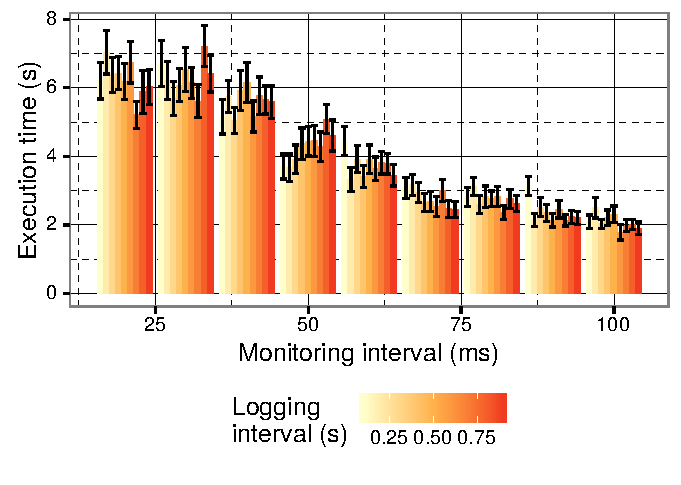
\includegraphics[width=\linewidth]{moca/moca_param.pdf}
        \caption{Execution time.}
        \label{fig:param_time}
    \end{subfigure}
    \begin{subfigure}{.73\linewidth}
        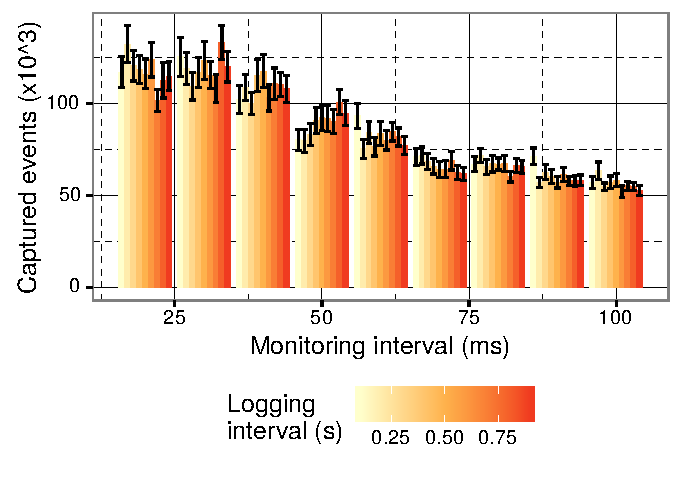
\includegraphics[width=\linewidth]{moca/moca_param_events.pdf}
        \caption{Number of captured events.}
        \label{fig:param_evts}
    \end{subfigure}
    \caption[Influence of Moca wakeup intervals.]{Influence of the wakeup intervals on \IS, class A.}
    \label{fig:param}
\end{figure}

We can see on the \fig{param_time} that the execution time increases when we reduce the monitoring wakeup interval.
At \SI{40}{ms} it seems to reach its worst level, thus we should keep it larger.
At \SI{50}{ms}, the default value we have chosen, the \fig{param_evts} shows that we obtain more than two thirds of the events captured at smaller intervals, which seems sufficient to us.
Regarding the logging interval, our experiments do not exhibit a clear trend.
Changing it seems to interfere with the system I/Os scheduler resulting in chaotic variations both in the execution time and the number of captured events.
The fact that variations in execution time result in matching variations in the number of captured events is due to the fixed length of monitoring intervals : the longer the execution, the more monitoring intervals there are and the more events the trace contains.
Overall these variations are not significant as all the confidence intervals intersect.
Finally we have chosen a logging interval of \SI{0.5}{s}, the median value, in order to avoid unnoticed effect caused by extremum values.

\subsection{Comparison to other memory trace collection tools}

Preliminary experiments showed us that \gls{Mitos} capture by default way less distinct pages than \gls{Tabarnac} and \gls{Moca}.
Thus, we tried to change \gls{Mitos} sampling period in order to make it capture as many pages as possible, we name this version MitosTun.
Surprisingly, \gls{Mitos} behavior regarding this sampling period is not monotonous, we had to try many different periods to find the proper one.

The default \gls{MemProf} distribution did not work with our experimental setup.
With the help of their support team\footnote{
    see issue at \href{https://github.com/Memprof/scripts/issues/1}{github.com/Memprof/scripts/issues/1}
}, we managed to make it work by disabling the library used to retrieve data structures names.
For the same reason as in the case of \gls{Mitos}, our study includes two versions of \gls{MemProf}: the default version and MemProfTun in which we have increased the sampling rate to its maximum.

Finally our evaluation also distinguishes \gls{Moca} (kernel module only) from MocaPin, which also retrieve the data structure information using a \gls{Pin} instrumentation.
In recent version of \gls{Moca}, the library that retrieve data structure information have been ported out of \gls{Pin}, as described in \sect{moca-design}.
Still it does the same work as the \gls{Pin} instrumentation but without the weight of \gls{Pin} therefore has a similar or lighter overhead.

We compare the different tools regarding two metrics, trace \emph{precision} and induced slowdown.
Regarding the trace \emph{precision}, the first experiment compares the tools using two criteria, the percentage of captured pages and the number of captured events.
We use \gls{Tabarnac} as a reference to compute the total number of pages accessed by the application because, by design, it traps all the memory accesses to compute the number performed in each page.
This metric is representative of the coverage of the memory space, that is the capacity of the tool to outline the whole memory area accessed by the application.
Regarding the number of captured events, we present the percentage relative to \gls{Moca}, as it is the tool that usually provides the more \emph{precise} traces.
We define one event as one timestamped access found in the trace file outputted by a tool.
According to this definition, \gls{Tabarnac} does not capture any event as it only keeps one counter per page and per thread without any temporal information.
Thus, \gls{Tabarnac} is excluded from this comparison.
The number of captured events is representative of the \emph{precision} of a monitoring tool, its capacity to keep track of all the evolutions of the access patterns during the course of the execution.
The idea is that, the more the tool captures events, the less it misses changes in the access patterns.
The second experiment compares the slowdown factor of the different tools.
All these experiments have been run on each of the \gls{NPB} on class A.

\begin{figure}[htb]
    \centering
    \begin{subfigure}{.73\linewidth}
        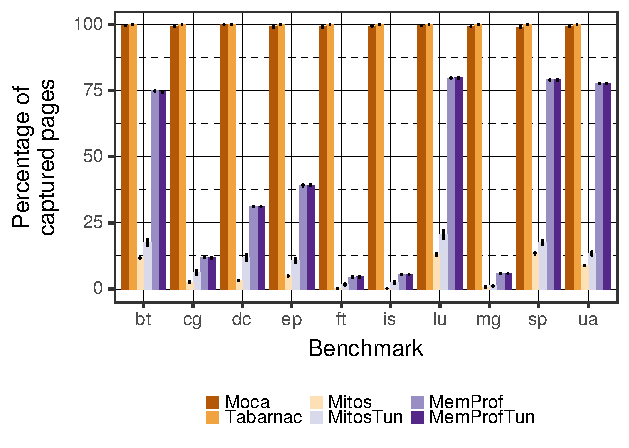
\includegraphics[width=\linewidth]{moca/moca_pages_intel.pdf}
        \caption{Percentage of captured pages.}
        \label{fig:pages}
    \end{subfigure}
    \begin{subfigure}{.73\linewidth}
        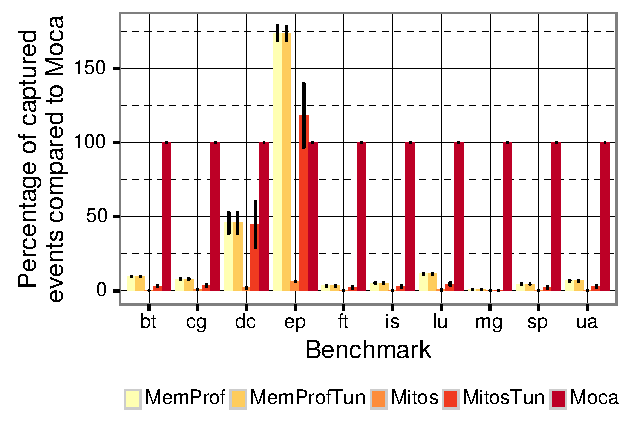
\includegraphics[width=\linewidth]{moca/moca_addr_intel.pdf}
        \caption{Percentages of events captured (compared to \gls{Moca}).}
        \label{fig:addr}
    \end{subfigure}
    \caption{Precision of the traces generated by each tool.}
    \label{fig:pages-addr}
\end{figure}

\fig{pages-addr} presents the results of the precision evaluation for the different tools.
The values used for \gls{Mitos}, MitosTun, \gls{Moca} and \gls{Tabarnac} result from runs on \texttt{Edel} machines, while \gls{MemProf} and MemProfTun values result from runs on \texttt{StRemi}.
We can see on \fig{pages} that \gls{Moca} captures almost as many pages as \gls{Tabarnac}.
Regarding their design they should capture as many pages.
Nevertheless, there is a slight bump in the number of pages used by applications monitored by \gls{Tabarnac} due to the Pin instrumentation.
Indeed, its JIT instrumentation recompiles the executable on the fly and changes the memory footprint (of the stack, mainly).
Thus, we can safely ignore these differences.

\gls{Mitos} usually collect less than \SI{12.5}{\%} of the pages, adding some fine tuning can almost double this number but it still misses most of the address space.
Regarding \gls{MemProf}, changing the default sampling rate does not seem to have any noticeable impact on the end result.
Both \gls{MemProf} and MemProfTun capture significantly more pages than \gls{Mitos} and MitosTun.
Nevertheless, for half of the studied applications it does not see more than \SI{50}{\%} of the addresses space.
Only for \BT, \LU, \SP and \UA, \gls{MemProf} manages to capture around \SI{75}{\%} of the accessed pages.
This is explained by the fact that all these benchmarks are using uniformly most of their address space, and that many pages are frequently accessed.
This is coherent with the fact that \gls{MemProf} is solely based on instructions sampling and only sees the most accesses pages.

From \fig{addr} we can see that, as expected, for almost every benchmarks, \gls{Moca} collects significantly more events than the other tools.
 The only benchmark for which \gls{Moca} is not the more \emph{precise} tool is \EP which is an Embarrassingly Parallel application with very few memory accesses.
This outlines the fact that \gls{Moca} captures events in an uniform way, timed by the monitoring interval.
On the contrary, the other tools might capture more events in a few hotspots presents in the application but miss sparse accesses during the rest of the execution.
For almost every other benchmarks both \gls{Mitos} (with or without tunning) and \gls{MemProf} hardly reach \SI{10}{\%} of the accesses collected by \gls{Moca}, the only exception is \DC for which \gls{MemProf} captures from \SI{25}{\%} to \SI{50}{\%} of the accesses collected by \gls{Moca}.

\begin{figure}[htb]
    \centering
    \begin{subfigure}{.73\linewidth}
        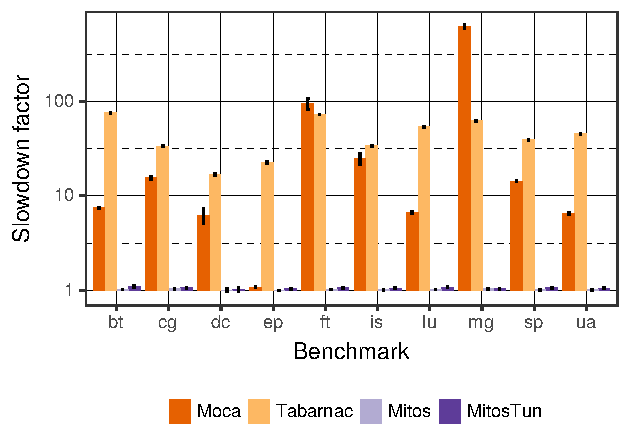
\includegraphics[width=\linewidth]{moca/moca_overhead_intel.pdf}
        \caption{Evaluation on \texttt{Edel} (Intel)}
        \label{fig:ovh-moca-Intel}
    \end{subfigure}
    \begin{subfigure}{.73\linewidth}
        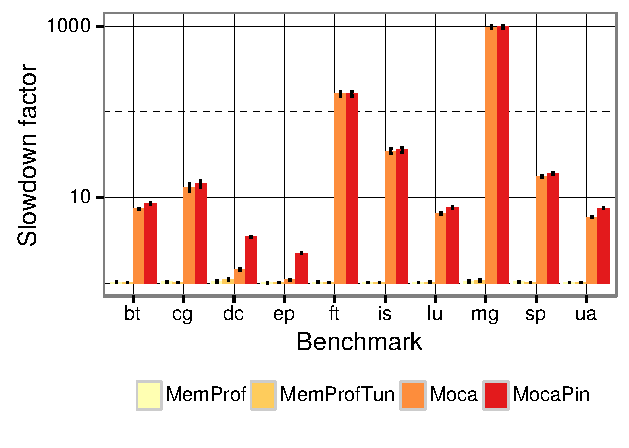
\includegraphics[width=\linewidth]{moca/moca_overhead_amd.pdf}
        \caption{Evaluation on \texttt{StRemi} (AMD)}
        \label{fig:ovh-moca-AMD}
    \end{subfigure}
    \caption[Slowdown factor of each tool.]{Slowdown factor of each tool.
    Y-axis in log scale.}
    \label{fig:ovh-moca}
\end{figure}

These results prove that most existing tools can miss a considerable part of
the address-space while \gls{Moca} guarantee that it traces covers all the accessed pages.
Furthermore they show that \gls{Moca} is the only existing tool able to provide a trace that is \emph{precise} enough to give an good overview of the memory use of an application.
In short, not only our tool provides a \emph{complete} trace at the granularity of the page but it is also significantly more \emph{precise} than the other existing tools.

\fig{ovh-moca} shows for each of the \gls{NPB}, the slowdown factor when instrumented by \gls{Moca} and the other existing tools on Intel (\fig{ovh-moca-Intel}) and AMD (\fig{ovh-moca-AMD}) Machines.
Notice that the Y-axis is in log scale.

From \fig{ovh-moca-Intel}, we can see that \gls{Mitos}, MitosTun overhead is almost negligible which is not the case for \gls{Moca} and \gls{Tabarnac}, this difference is explained by the results of the previous experiment, as these tools usually collects less than \SI{10}{\%} of the accesses collected by \gls{Moca} and miss a significant part of the address space.

We can classify the benchmarks into three groups: for \BT, \CG, \DC,  \EP, \LU, \SP and \UA, \gls{Moca} is significantly faster than \gls{Tabarnac}.
This set of benchmarks is interesting as it is made of varied application profiles as we can see in \tbl{NPB}.
Indeed, if \EP is mostly doing parallel computation with only a few number of memory accesses, \CG is described as memory intensive, \BT, \LU as well as \SP are linear algebra solvers with regular memory access patterns, and both \UA and \DC contain \emph{unstructured computation, parallel I/O and data movement}.
Furthermore, \DC has a considerable memory footprint as described in \tbl{NPB}.
The second group only contains memory intensive benchmarks (\FT and
\IS). For this group, \gls{Moca} is as good as \gls{Tabarnac} or a bit faster, probably
because the balance between computations and memory accesses hides the
overhead of the instrumentation.

For the last benchmark: \MG, \gls{Moca} is significantly slower than \gls{Tabarnac}.
By looking at our experiment logs, we found that \MG generates a lot of conflicts in the hash map used by \gls{Moca} to store false page faults.
This issue is caused by applications that perform a very large number of sparse accesses to a large working set.
This is not usual as parallel applications are often optimized to make memory accesses as local as possible in order to take advantage of all the levels of the memory hierarchy.
Thus, we consider this benchmark as a pathological case.
A solution could be to increase the size of this hash map, which is not always possible as memory space in the kernel is limited (and these experiments have been run with the largest hash map we could use).
Another easier solution would consist in working on a smaller instance of \MG and see if the trace is still useful.
Although the results are not presented here, we have run \gls{Moca} on \MG with a smaller size (W) and we have been able to confirm that the performance becomes comparable to \gls{Tabarnac} in this case.

\fig{ovh-moca-AMD} shows the results of the evaluation on the AMD machine
(\texttt{StRemi}). On this machine, \gls{Moca} overhead is quite similar to the one
obtained on \texttt{Edel}.
\gls{MemProf} exhibits a slowdown factor comparable to \gls{Mitos} while
providing traces a little more \emph{precise}. Nevertheless, they are still \emph{incomplete} and
way less \emph{precise} than \gls{Moca} traces. Obviously MemProfTun has the same
overhead as \gls{MemProf} as it captures the same amount of data.

Finally, we can see, as expected, that adding one execution with a Pin instrumentation to retrieve data structures information (MocaPin) only adds a small overhead to the whole \gls{Moca} execution.
For several benchmarks this difference is so small that we cannot distinguish it from \gls{Moca} usual overhead.

\subsection{Results and discussion}

We have tested \gls{Moca} with various applications and using several parameters.
Our experiments, show that \gls{Moca} has a good behavior for a wide range of parameters and helped us defining their default values.
Our experiments also show that, with these parameters, \gls{Moca} provides significantly more precise traces than state of the art tools.
Of course, because of this increased precision, \gls{Moca} is slower than two of these tools, \gls{MemProf} and \gls{Mitos}.
Nevertheless, compared to the only other tool able to collect a superset of the memory space, \gls{Tabarnac}, \gls{Moca} exhibit a decent overhead.
Collecting such a superset with \gls{MemProf} and \gls{Mitos}, and provide the same guarantee, would require to sample all the memory instructions, which is not possible.
At the end of the day, \gls{Moca} is the only tool able to provide a detailed trace with temporal, spacial and sharing information while providing guarantees about the information lost during the sampling.

\section{Conclusions}
\label{sec:moca-cncl}

We addressed the issue of memory accesses collection for multithreaded applications.
This is a key challenge in high performance computing as memory is often a performance bottleneck.
Memory traces can be used at runtime to improve data locality or offline by developers to understand and improve the memory behavior of their applications and, therefore, their performances.
For online analysis the trace \emph{precision} is limited by the volume of data that can be analyzed in real time, but for offline usage, highly accurate traces can provides a better understanding of the application memory behavior.

Our first attempt at collecting memory traces, \gls{Tabarnac}, is designed specifically for \gls{NUMA} related issue.
It relies on a custom memory tracer based on the Pin dynamic binary instrumentation tool which records the number of memory reads and writes performed by all threads for each data structure.
The advantage of instrumentation is that it is the most accurate and portable way to generate memory traces.
Despite the overhead caused by the instrumentation, \gls{Tabarnac} is efficient enough to analyze even huge applications in a reasonable time.

We analyzed two parallel applications with \gls{Tabarnac}: \emph{Ondes3D}, a real life application that
simulates seismic waves, and \IS from the \gls{NPB} which is known for being memory intensive with a random memory access pattern.
For both applications, \gls{Tabarnac} helped us understand their performance issues.
Using this knowledge, we proposed simple code modifications to optimize the memory behavior resulting, for each application, in significant speedups compared to the original version (up to $60\%$ speedup).
Improvements were also substantially higher than those provided by automated tools.
Yet, \gls{Tabarnac} traces are not \emph{precise} as they only contains a global overview of the memory sharing patterns without temporal information.
Therefore they only enable the observation of a limited number of memory related issues.

Our second memory trace collection tool, \gls{Moca} addresses this challenge.
It  collects \emph{precise}, \emph{complete} and \emph{detailed} memory traces.
While existing tools rely on \emph{incomplete} hardware sampling to provide such traces at a lower cost, \gls{Moca} provides a \emph{complete} trace, that contains all the accessed areas, at the granularity of the page.
Moreover, \gls{Moca} traces not only contain all the pages that are accessed during the execution, but also, for each trapped access, temporal, spatial and sharing information: accesses are timestamped and recorded along with their thread number, CPU number, and kind.
While \gls{Moca} works at the page granularity, it stores the exact address of each intercepted accesses.
Therefore, it also provides an \emph{incomplete} trace at the granularity of the Byte, similar to traces collected by instructions sampling.
Furthermore, \gls{Moca} is also able to relate accesses to data structures of the application by combining this efficient trace collection system with an examination of the application binary.

Most state of the art tools are relying on hardware technologies such as \gls{Intel} \gls{PEBS} or \gls{AMD} \gls{IBS}, and embed vendor (or processor) dependent code making them hard to maintain and not portable.
On the contrary, \gls{Moca} is based on page faults interception as well as false page faults injection mechanisms and does not use any architecture dependent code.
It can work on any \gls{Linux} kernel from $3.0$ only by loading a module and without any kernel modification.

Several tools use page faults interception to retrieve information about the memory use.
As information provided by only intercepting regular page faults is not always \emph{precise} enough, a few tools also inject false page faults on a regular basis to increase the trace \emph{precision}.
To our knowledge, all the existing tools relying on these mechanisms uses the collected data online and, thus, do not have to manage and store a large volume of data.
\gls{Moca} is the first tool able to generate and store \emph{complete} and \emph{precise} memory traces for offline analysis.

We evaluated \gls{Moca} and \gls{Tabarnac} by comparing them to two state of the art tools: \gls{Mitos} (the collection tool from \gls{MemAxes}) and \gls{MemProf}.
Both of these tools were evaluated with their default parameters and with some fine tunning of our own.
For this comparison, we evaluated two criteria: the \emph{precision} of the trace and the runtime overhead.
We ran our evaluation on the \gls{NPB} which are representative of multiple kinds of applications from simple kernels to realistic ones.
Our evaluation has exposed the fact that the tools relying on hardware sampling miss a large part of the address space.
It has also shown that \gls{Moca} is able to provide both a \emph{complete} trace at the page granularity and a sampling at the Byte granularity significantly more \emph{precise} than the other sampling based tools.
Generating comparable traces using \gls{MemProf} or \gls{Mitos} would require to sample more memory instructions than the hardware can.
Finally, \gls{Moca} overhead is more important than the overhead of sampling based tools but usually lower than the one induced by \gls{Tabarnac}.

The visualization and exploitation of these memory traces is another challenge.
Indeed, not only theses traces contains an important volume of data, but they are spread over several dimensions.
The most obvious ones are the address space and the time.
Yet, the threads responsible for the accesses also represent a dimension of the trace.
Moreover, the \gls{CPU} location of the access is not necessarily bound to the threads, hence it is one more dimension.
Finally, the type of access (read or write, private or shared) is yet another dimension.
Several of these five dimension can be observed from different point of view, for instance the address space can be physical or virtual,  and the time can be seen either as a discrete sequence of timestamp or as the result of the code.
In summary, our traces contain at least five dimensions, therefore designing meaningful and intuitive visualization is far from being trivial.

% vim: et si sta lbr  sw=4 ts=4 spelllang=en_us
